\chapter{Elementos de Aprendizaje Automático}\label{chapter:MLIntro}

Este capítulo provee una breve introducción a los elementos y conceptos del aprendizaje automático abordados a lo largo del trabajo. En su mayoría, corresponden a conceptos esenciales del área y servirán de base para el modelo seleccionado como propuesta de solución. 

\section{Aprendizaje automático}

El aprendizaje automático es el subcampo de las ciencias de la computación y una rama de la inteligencia artificial, cuyo objetivo es desarrollar técnicas que permitan que las computadoras aprendan. Por moderno que pueda parecer, su origen se remonta al año 1950 cuando Alan Turing creó el "Test de Turing". Para pasar el test, una máquina debía engañar a un humano haciéndole creer que se encontraba delante de un humano en lugar de un ordenador.

El aprendizaje automático abre las puertas a un nuevo paradigma de programación. La programación clásica se entiende como un conjunto de reglas diseñadas por una persona con el fin de obtener unas respuestas que cumplan dichas reglas a partir de unos datos de entrada. El aprendizaje automático, en cambio, se encarga de obtener el conjunto de reglas más efectivas que relacionan los datos de entrada con las respuestas que se esperan obtener a través del aprendizaje. Luego, estas reglas se pueden aplicar a nuevos datos para producir respuestas asociadas a los mismos. Esta comparación se muestra en la figura \ref{PCvsML}.

\begin{figure}[!h]
	\centering
	
	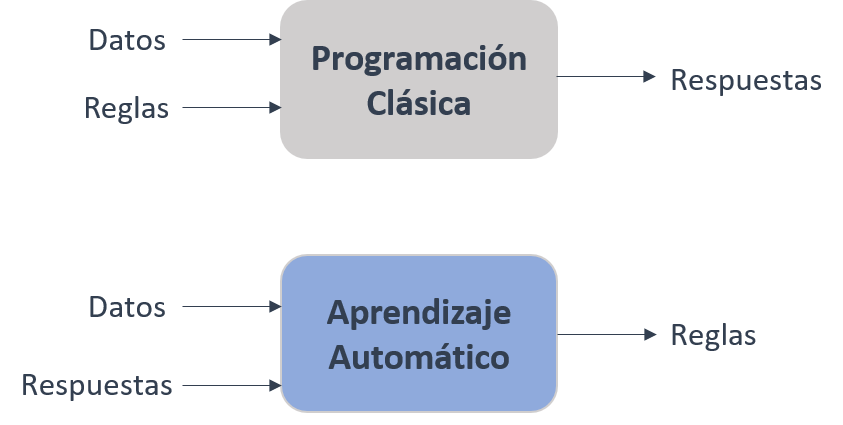
\includegraphics[width=3in]{Graphics/PCvsML.png}
	
	\caption{ \small{Programación clásica frente al aprendizaje automático.}}
	
	\label{PCvsML}
	
\end{figure}


El objetivo en el aprendizaje automático es seleccionar una función o hipótesis que se ajuste de manera óptima a ejemplos futuros o nuevos. Los parámetros de la función se ajustan durante el entrenamiento mediante un algoritmo de optimización conocido como descenso del gradiente. En esencia, transforma los datos de entrada a una salida que tiene una representación significativa, mediante un proceso llamado \textbf{aprendizaje}. 

Las tareas en este terreno, usualmente se describen en términos de cómo se procesa la entrada al sistema. Por lo general, se expresa como un vector $x \in \mathbb{R}$ donde cada componente del mismo constituye una característica. Por ejemplo, las características de una imagen pueden ser los valores de sus píxeles. Un sistema de aprendizaje automático se basa en un proceso de \textbf{entrenamiento} en lugar de ser programado explícitamente. Gracias a ello, permite encontrar una estructura estadística en los datos de entrada que dará lugar a nuevas reglas para automatizar la tarea en cuestión. En la siguiente sección se incluyen algunas tareas que se pueden resolver con técnicas de este dominio y que serán mencionadas a lo largo del documento. 

\subsection{Tareas de ML}\label{1-MLtareas}

Una tarea de aprendizaje automático es el tipo de predicción o inferencia que se realiza, en función del problema o la pregunta que se formula, y los datos disponibles. Las mismas se basan en patrones que pueden aparecer en los datos en lugar de programarse explícitamente. A continuación se muestran algunas de ellas.

\subsubsection{Clasificación}\label{1-Clasif}
 Su objetivo es clasificar la entrada del programa en una de las $k$ categorías posibles según el problema. Para resolverlo, el algoritmo de aprendizaje produce una función $f:\mathcal{R}^n \rightarrow \{1, ..., k\}$. Existen otras variantes de clasificación, por ejemplo, cuando $f$ devuelve una función de distribución de probabilidad sobre las $k$ categorías \cite{BengioGood}.
 
 \subsubsection{Regresión}\label{1-Regres}
 El algoritmo de aprendizaje reporta una función $f: \mathcal{R}^n \rightarrow \mathcal{R}$ para predecir un valor numérico a partir de la entrada. Un ejemplo de regresión es la predicción de los precios futuros en el mercado \cite{BengioGood}.

\subsubsection{Traducción automática}\label{1-TradAut}
 Del inglés \textit{machine translation}. La entrada consiste en una secuencia de símbolos en un determinado lenguaje, y el algoritmo la convierte a una secuencia de símbolos pero de otro lenguaje \cite{BengioGood}. Comúnmente se aplica en lenguajes naturales, por ejemplo para traducir del inglés al francés \cite{SutskeverSeq2seqNN, BahdanauAlignTrans}.
 
 \subsubsection{Detección de anomalías}\label{1-DetAnom}
 
 Es la identificación de elementos raros, eventos u observaciones que generan sospechas al diferenciarse significativamente de la mayoría de los datos. Normalmente, los datos anómalos se pueden conectar a algún tipo de problema o evento raro como, por ejemplo, fraude bancario, problemas médicos, defectos estructurales, equipo defectuoso, etc \cite{BengioGood}.
 
 %\subsubsection{Denoising}\label{1-Denois}
 
 %En este tipo de tareas, la entrada $x$ se altera mediante un proceso que añade ruido a la información contenida en sus valores, obteniendo así $\tilde{x} \in \mathcal{R} $. El algoritmo debe predecir $x$ a partir de su versión $\tilde{x}$, o más general, predecir la distribución de probabilidad condicional $p(x| \tilde{x})$.
 
 \subsubsection{Estimación de densidad(función de probabilidad)}\label{1-EstimDen}
 
En el problema de estimación de densidades, el algoritmo aprende una función $p_{model} : \mathbb{R}^2 \rightarrow \mathbb{R}$ de donde $p_{model}(x)$ se interpreta como la función de densidad (si $x$ es continuo) o una función de probabilidad (si $x$ es discreto) en el espacio donde se encuentran los elementos de entrada. Esta tarea permite capturar explícitamente una distribución, que además, podrá ser usada en otros fines. Por ejemplo, si se tiene una función de probabilidad ya estimada $p(x)$, la misma se puede usar para obtener un valor faltante $x_i$ a partir del resto de valores ya conocidos $x_{-i}$, dado por $p(x_i| x_{-i})$. 

\subsubsection{Reducción de dimensión}\label{1-RedDim}

Se define como una forma de convertir un conjunto de datos de dimensiones elevadas en un conjunto de datos de dimensiones menores, asegurando que la información proporcionada sea similar en ambos casos. Esta técnica es especialmente útil como paso intermedio en los modelos predictivos, ya que son conjuntos de datos que contienen un elevado número de características de entrada, y hace más complicada su función. Ejemplo de ello son los modelos \textit{autoencoders} que se abordan en este trabajo \cite{Chollet}.

\subsubsection{Extracción de características}\label{1-ExtCar}
Consiste en utilizar las representaciones aprendidas por un programa entrenado previamente para extraer características interesantes en nuevas muestras o datos. Básicamente, es un proceso de reducción de dimensión mediante el cual un conjunto inicial de datos se reduce a grupos más manejables para su procesamiento. Se usan para tareas de clasificación de imágenes donde el conjunto de datos es pequeño \cite{Chollet}.\\


Existen además otros tipos de tareas cuya solución es posible en este ámbito. Las listadas anteriormente son una muestra importante que están relacionadas con la investigación realizada en este trabajo.   

\subsection{Ramas dentro del aprendizaje automático}
\label{1-MLramas}

 Previamente se presentaron varios tipos de tareas específicas del aprendizaje automático. La definición de las mismas está relacionada con las características y procesamiento de los datos de entrenamiento \cite{Chollet}. En términos generales, los algoritmos de ML se pueden clasificar como no supervisados o supervisados según el tipo de experiencia que se les permite tener durante el proceso de aprendizaje \cite{BengioGood}. Clásicamente dichos algoritmos se separan en tres categorías descritas a continuación.
 
 \subsubsection{Aprendizaje supervisado}\label{1-MLsupervisado}
 El algoritmo se entrena con variables que incluyen los valores que se desean predecir; a estos valores conocidos se les llama $"$ etiquetas $"$. Su objetivo es crear una función capaz de predecir el valor correspondiente a cualquier objeto de entrada válida después de haber visto una serie de ejemplos, los datos de entrenamiento. Para ello, tiene que generalizar las situaciones no vistas previamente a partir de los datos presentados. La salida de la función puede ser un valor numérico (como en los problemas de regresión) o una etiqueta de clase (como en los de clasificación).
 
 \subsubsection{Aprendizaje no supervisado}\label{1-MLnosupervisado}
 
 Consiste en encontrar patrones interesantes en los datos de entrada sin necesidad de observar cuál es la salida.  Por lo tanto, el  objetivo es extraer información significativa de los datos, los cuales carecen de etiqueta y cuya estructura es desconocida. Existen dos tipos de problemas característicos en el aprendizaje no supervisado: el agrupamiento o \textit{clustering}, y la reducción de dimensión \cite{Chollet}. El agrupamiento se encarga de crear conjuntos de objetos de características similares, mientras que la reducción
 de dimensión busca información redundante en los datos para reducir el número de variables y así mejorar el rendimiento computacional
 
 \subsubsection{Aprendizaje reforzado}\label{1-RL}
 El aprendizaje reforzado (\textit{reinforcement learning}, RL) es una forma de aprendizaje automático basado en un sistema de recompensas y castigos en el que un agente busca las decisiones óptimas para obtener la máxima recompensa tanto a corto como a largo plazo. A diferencia del aprendizaje no supervisado, el aprendizaje reforzado trata de maximizar la función de recompensa (\textit{reward function}) en lugar de encontrar ciertos patrones ocultos en un conjunto de datos no etiquetados. El aprendizaje reforzado se hace cargo de una gama cada vez más amplia de aplicaciones del mundo real: vehículos autónomos, robótica, gestión de recursos, educación, etc \cite{Chollet}.\\
 
 %Cada algoritmo de aprendizaje reforzado debe seguir una política (policy) para decidir qué  decisión tomar en función del estado en el que se encuentre. No obstante, esta política   puede no seguirse en la etapa de aprendizaje. Aquellos algoritmos cuya regla de actualización realiza la acción que traerá el máximo beneficio a pesar de que la política actual  restrinja dicha acción, se denominan algoritmos \textit{off-policy}.
 
 %TODO: Esto es porque en el estado del arte se menciona una aplicación con este algoritmo
 
 %Q-learning es un algoritmo off-policy de aprendizaje reforzado que busca la mejor acción dado  el estado actual. Se considera off-policy porque la función aprende de las acciones que están  fuera de la política actual, como por ejemplo las acciones aleatorias. El objetivo es aprender la  política que maximice la recompensa total. La Q de Q-learning viene de quality, que en este caso mide lo útil que ha sido una acción para ganar una recompensa futura
 
 Un problema importante en el aprendizaje automático en general, es la tensión entre la optimización y generalización. La \textbf{optimización} se refiere al proceso de ajustar un modelo para obtener el mejor rendimiento posible en los datos de entrenamiento (aprendizaje), mientras que la \textbf{generalización} se refiere a qué tan bien se desempeña el modelo entrenado en los datos que nunca ha visto antes. 
 
 El objetivo es obtener una buena generalización, pero si no es controlada es posible que el modelo se ajuste en función de sus datos de entrenamiento solamente. Los procesos y conceptos involucrados para lograr este equilibrio se argumentan en la siguiente sección.
 
 %MEJORAR TRANSICIÓN
 
 \section{Fundamentos del aprendizaje automático}
 
 En este apartado se presentan los fundamentos para comprender la forma en la que las máquinas aprenden. Para ello, se explican los conceptos de función de costo y el método de descenso por gradiente. Posteriormente, se muestran los principales errores o problemas que surgen a la hora de realizar un modelo de ML: la varianza (variance), el sesgo (bias), el sobreajuste (overfitting) y el subajuste (underfitting). Por último, se explican los pasos a seguir para desarrollar e implementar una solución con ML.
 
 \subsection{Aprendizaje}\label{1-Learning}
 
 El aprendizaje en un sistema de ML consiste en el ajuste de los parámetros de un modelo en función de los datos recibidos. Este conjunto de datos contiene variables tanto independientes como dependientes. Las variables  independientes (\textbf{características}) son aquellas usadas por el algoritmo para generar un modelo que prediga lo mejor posible las variables dependientes. Por otro lado, las variables dependientes (\textbf{etiquetas}) son el resultado de una correlación entre las variables independientes, por lo que deben ser predichas por el modelo implementado. 
 
 El modelo debe estar lo suficientemente ajustado a los datos de entrada, pero también debe tener la suficiente consistencia como para dar un buen resultado ante la introducción de datos diferentes. Para ello, el conjunto de datos se divide en 3 subconjuntos: los datos de entrenamiento (\textbf{training set}), con los que se entrenan los modelos candidatos; los datos de validación (\textbf{validation set}), para evaluar los modelos candidatos y seleccionar el mejor; y los datos de prueba (\textbf{test set}) para realizar una evaluación final del mejor modelo \cite{PeterNorvig}.
 
 Una vez se tienen los datos se establece una hipótesis, es decir, encontrar una ecuación que se aproxime lo mejor posible al comportamiento real del fenómeno que se está  modelando. Esta ecuación relaciona los datos de entrada y los parámetros del modelo con la salida y se conoce como \textbf{función de pérdida}. Se encarga de recopilar el error entre la variable dependiente que se quiere determinar y la hipótesis, en función de los parámetros del modelo.
 
 La diversidad de modelos y funciones de pérdida en ML obliga a encontrar soluciones para las funciones no-convexas, es decir, para aquellas que tienen más de un mínimo.  El método de \textbf{Descenso por Gradiente} aprovecha el cálculo de la derivada para encontrar los mínimos locales, ya que la derivada indica el valor de la pendiente en un punto determinado. El gradiente proporciona información sobre cuánto varía la función por cada unidad que varía cada variable en el punto considerado. Un gradiente positivo indica la dirección por la cual avanzar si se quisiera encontrar un máximo
 (Ascenso del Gradiente). En este caso, se explora el espacio en el sentido contrario al gradiente, ya que el objetivo es encontrar un mínimo de la función.
 
 \subsection{El error y los problemas de ajuste}\label{1-Ajuste}
 
 La precisión y la capacidad de generalizar son aspectos clave a la hora de realizar un modelo de ML solo que, lamentablemente, es imposible conseguir que un modelo esté libre de errores por completo. Comprender las principales fuentes de error ayuda a prevenir dos de los problemas más habituales en el ajuste de parámetros: el sobreajuste (\textbf{overfitting}) y el subajuste o falta de ajuste (\textbf{underfitting}).
 
 Los errores principales en la predicción de un modelo, y que están asociados al algoritmo empleado, son la varianza y el sesgo (bias). El error de varianza está relacionado con el grado en el que la función objetivo cambia según los datos de entrenamiento proporcionados. El error de sesgo es la diferencia entre los valores reales y la predicción que espera el modelo. El error total es una combinación de varianza y sesgo, por lo que para minimizarlo es imprescindible lograr una baja varianza y un bajo sesgo. Sin embargo, la estrecha relación entre la varianza y el sesgo hace que disminuir uno de ellos
 implique aumentar el otro.
 
 El subajuste (underfitting) se refiere a un modelo con un nivel de complejidad muy bajo que no tiene la precisión suficiente como para alcanzar un ajuste adecuado debido a su alto sesgo. Puede ocurrir cuando el conjunto de datos de entrenamiento no es suficiente, o cuando se utiliza un modelo lineal para ajustar datos no lineales. Por otra parte, el sobreajuste (overfitting) se produce cuando el nivel de complejidad es elevado y, por lo tanto, el modelo no tiene la capacidad de generalizar su comportamiento ante diferentes datos de entrada. Sucede cuando el modelo recoge el ruido de los datos de entrenamiento y, en consecuencia, aumenta mucho su varianza.
 
 \subsection{Etapas de un proyecto de ML}\label{1-etapas}
 
 Una vez presentados los principios básicos del ML, es conveniente conocer el procedimiento para dar solución a problemas reales usando estas técnicas. Un proyecto de ML no se centra únicamente en elegir un modelo y entrenarlo, sino que, como todo proyecto, cuenta con una serie de etapas o pasos a seguir para aumentar sus probabilidades de éxito. A continuación, se describen ocho etapas genéricas \ref{etapasML} para llevar a cabo un proyecto de ML.
 
  \begin{figure}[!h]
 	\centering
 	
 	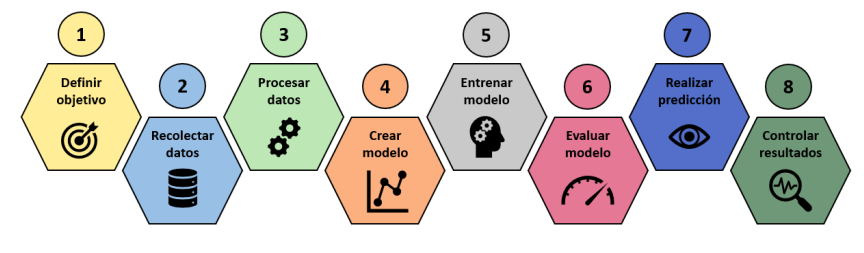
\includegraphics[width=4in]{Graphics/etapasML.png}
 	
 	\caption{ \small{Etapas genéricas de un proceso de ML.}}
 	
 	\label{etapasML}
 	
 \end{figure}

La primera etapa consiste en entender el problema que se quiere resolver, ya que gran parte de las decisiones tomadas a lo largo del proyecto dependerán de lo bien que se haya comprendido el contexto. Para ello es necesario definir unos objetivos claros, medibles y alcanzables en un período determinado de tiempo. En este punto se clasifica el problema (supervisado, no supervisado, etc.) e incluso se elige el tipo de modelo que se va a entrenar.

En la segunda etapa se define la cantidad y el tipo de datos necesarios, así como el origen de dichos datos. La calidad de los datos tiene un impacto directo en el funcionamiento del modelo. Por tal motivo, es necesario desarrollar una tercera etapa de tratamiento y procesamiento de los datos, cuyo objetivo es visualizar y analizar cuáles son las variables que mejor representan aquello que se quiere predecir. Además, los datos requieren un formato determinado para poder procesarse de la manera más sencilla posible. Para ello debe se debe tener en cuenta las características de la arquitectura empleada y la representación seleccionada para los datos. En esta tercera etapa se incluyen dos procedimientos que tienen lugar en este trabajo y consisten en lo siguiente: 
	
	\begin{description}
		\item[Vectorización:] todas las entradas y etiquetas deben ser vectores con valores reales.
		
		\item[Normalización:] una vez vectorizados los datos, deben cumplir además que sus valores se encuentren en el intervalo $[0, 1]$.
	\end{description}

Una vez hecho esto, se divide el conjunto de datos en los 3 subconjuntos mencionados anteriormente. 

Aunque en el primer paso ya se conoce el tipo de problema, es en la etapa cuatro donde se define por completo el modelo que mejor se ajusta al problema: regresión lineal, árboles de decisión, red neuronal, k-vecinos más cercanos, etc. La solución propuesta en este trabajo contempla dos modelos de redes neuronales conocidos como \textit{autoencoder} y \textit{variational autoencoder}.

La quinta etapa se dedica al entrenamiento del modelo a partir de los datos de entrenamiento. Los parámetros se ajustan automáticamente por el algoritmo seleccionado a medida que se entrena el modelo. En la etapa número seis se verifica la precisión del modelo mediante la introducción de los datos de prueba, que son datos distintos a los del conjunto de entrenamiento. También se evalúan los errores que hacen que el modelo no generalice bien con el fin de elegir la solución más conveniente: adquirir más datos, usar un modelo más simple, usar uno más complejo, comprender mejor el problema, etc. A esta etapa también se la conoce como Parameter Tuning (configuración de parámetros), pues consiste en ajustar los parámetros del modelo para mejorar los resultados obtenidos.

Cuando se alcanza el nivel de error deseado, el modelo queda validado y puede pasarse a la penúltima etapa, que es la unión entre la simulación y el mundo real. Se trata de integrar el modelo en un sistema real con el que pueda comunicarse. Por último, la etapa número ocho pone fin al proceso con la monitorización de los resultados. Es necesario asegurar que el modelo aporta un alto valor predictivo y, lo más importante, que
cumple con los objetivos marcados en la primera etapa.

El aprendizaje automático comenzó a florecer en la década de 1990. Según \textit{Chollet et al.} \cite{Chollet}, una tendencia impulsada por la disponibilidad de \textit{hardware} más rápido y también conjuntos de datos de mayor dimensión. A diferencia de la estadística, el aprendizaje automático tiende a tratar con conjuntos de datos más grandes y complejos (como un conjunto de millones de imágenes, cada una de ellas formada por decenas de miles de píxeles) cuyo análisis estadístico clásico, como el análisis bayesiano, no sería practicable. Como resultado, el aprendizaje automático, y especialmente el aprendizaje profundo, exhibe poca teoría matemática. Esta disciplina, conocida en inglés como \textit{deep learning}, se introduce en la siguiente sección.


  
 \section{Aprendizaje profundo}\label{1-DeepLearn}
 
 Existe un área específica del aprendizaje automático llamada aprendizaje profundo (\textit{deep learning}), que se basa en algoritmos de aprendizaje en múltiples niveles de representación y de abstracción con el fin de modelar relaciones más complejas entre los datos. Los niveles se corresponden con distintos niveles de conceptos, y a cada uno, le corresponde una capa dentro de una secuencia formada por capas. Esta idea de representaciones sucesivas es lo que da el nombre de “profundo” a este tipo de aprendizaje, siendo la profundidad del modelo el número de capas que contiene \cite{deng2014deep}.
 
 En el aprendizaje profundo, estas representaciones por capas forman una red neuronal (\textit{neural network}) que constituyen un conjunto estructurado de neuronas \ref{RedNeuronal}. Estos términos provienen de la neurobiología ya que estas redes se inspiran en el funcionamiento del cerebro. Las capas están formadas por un número determinado de neuronas, donde cada neurona recibe información de la capa anterior por medio de estímulos externos a través de sus conexiones de entrada. 
 
 Las neuronas realizan cálculos internamente y sobre ellas se usa una función de activación para propagar la salida de los nodos o neuronas de la capa actual hacia la siguiente capa. Se trata de funciones que producen la activación de la neurona. Este tipo de funciones permiten incorporar la modelación de relaciones no lineales en los datos de entrada a la red.
 
 La función de activación \textit{relu} es la más utilizada en el aprendizaje profundo \cite{Chollet} y se define como $ReLU(z) = max(0, z)$. Otro ejemplo es la función $sigmoid$ que se determina mediante la función $\sigma(z) = \frac{1}{1 + e^{-z}}$. Ambas funciones se emplearon en los modelos implementados en este trabajo.
 
 
 
 % devuelven un valor de salida que se transmite a las neuronas de la capa siguiente. En la última capa, la salida es la predicción buscada \cite{Chollet}.
 
 \begin{figure}[!h]
 	\centering
 	
 	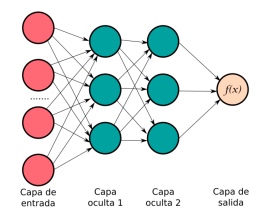
\includegraphics[width=2.55in]{Graphics/redNeuronal.png}
 	
 	\caption{ \small{Arquitectura básica de una red neuronal.}}
 	
 	\label{RedNeuronal}
 	
 \end{figure}

%Sin embargo, para llegar a una buena predicción, la red debe ser capaz de minimizar el error entre la predicción y el valor esperado mediante el autoajuste de los parámetros del modelo.

La especificación de lo que hace una capa con sus datos de entrada se almacena en los \textbf{pesos} de la capa, que en esencia, son un conjunto de números. En términos técnicos, se dice que la transformación implementada por una capa se \textbf{parametriza} por sus pesos (los pesos también se denominan parámetros de una capa) \ref{RedLoss}. En este contexto, aprender significa encontrar un conjunto de valores para los pesos de todas las capas en una red, de modo que la red transforme correctamente la entrada a su objetivo asociado.

El aprendizaje ocurre al extraer lotes (\textit{batches}) aleatorios de muestras de datos y sus
etiquetas, y calcular el gradiente de los parámetros de la red con respecto a la pérdida en el lote. Luego, los parámetros de la red se mueven un poco en el
dirección opuesta al gradiente.

Para controlar el valor de la salida de la red, se mide qué tan lejos se encuentra la misma de la respuesta deseada mediante la \textbf{función de pérdida}, también llamada función objetivo. La función de pérdida toma las predicciones de la red y el verdadero objetivo (lo que deseaba que produjera la red) y calcula una medida de distancia, capturando qué tan bien ha funcionado la red para cada uno de los ejemplos de entrada. 

 Todo el proceso de aprendizaje es posible gracias al hecho de que la red neuronal constituyen cadenas de operaciones vectoriales \textbf{diferenciables} Chollet et al. \cite{Chollet} y, por lo tanto, es posible aplicar la regla de derivación de la cadena para encontrar la función de gradiente que transforme a los parámetros actuales y al lote actual de datos, a un valor de gradiente.

 \begin{figure}[!h]
	\centering
	
	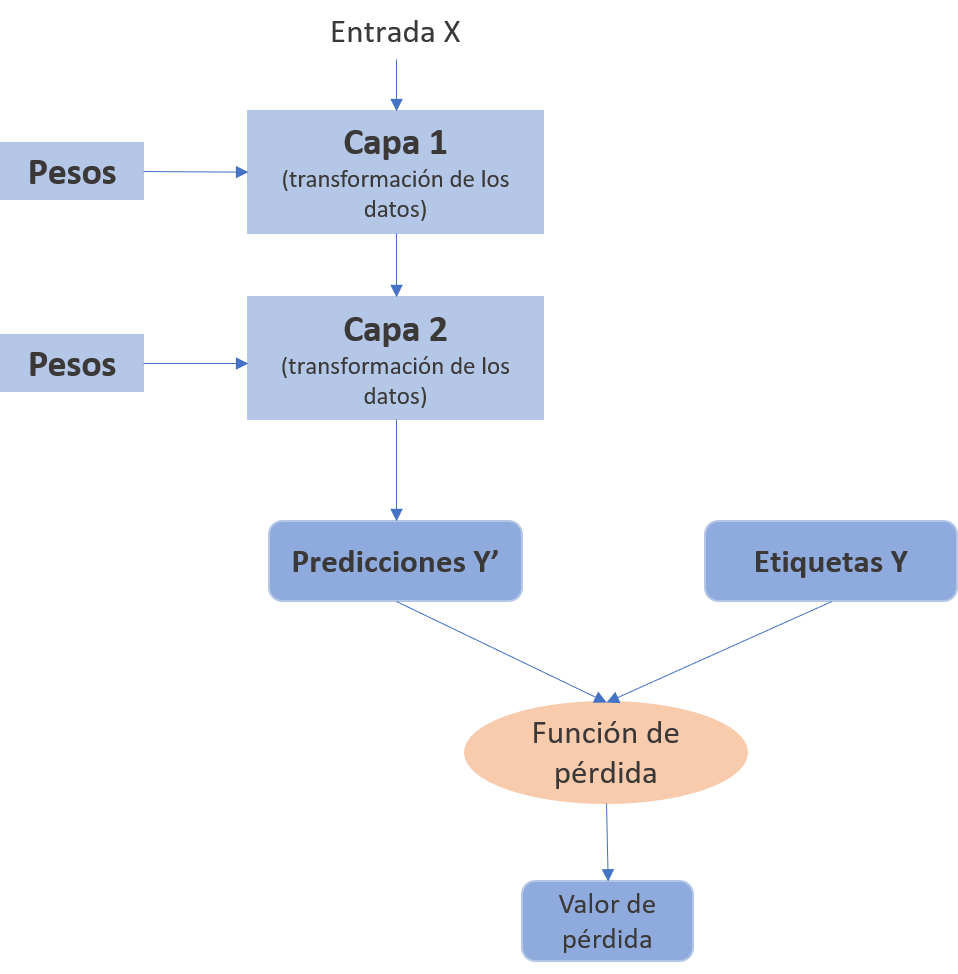
\includegraphics[width=3.8in]{Graphics/redLoss.png}
	
	\caption{ \small{Red neuronal parametrizada por sus pesos y con función de pérdida para evaluar la calidad de la salida.}}
	
	\label{RedLoss}
	
\end{figure}

El truco fundamental en el aprendizaje profundo es utilizar esta medida como una señal de \textbf{retroalimentación} para ajustar el valor de los pesos, en una dirección que reducirá la medida de pérdida para el ejemplo actual. Este ajuste es el trabajo del \textbf{optimizador}, que implementa lo que se conoce como algoritmo \textbf{Backpropagation} \cite{Chollet}.

En la literatura existen varios algoritmos de optimización basados en el descenso por gradiente. Entre los más conocidos se encuentran los algoritmos de optimización \textit{Adam} y \textit{RMSProp} \cite{BengioGood}. Este último utiliza una tasa de aprendizaje adaptativa en lugar de tratar la tasa de aprendizaje como un hiperparámetro. Esto significa que la tasa de aprendizaje cambia con el tiempo.  


\begin{figure}[!h]
	\centering
	
	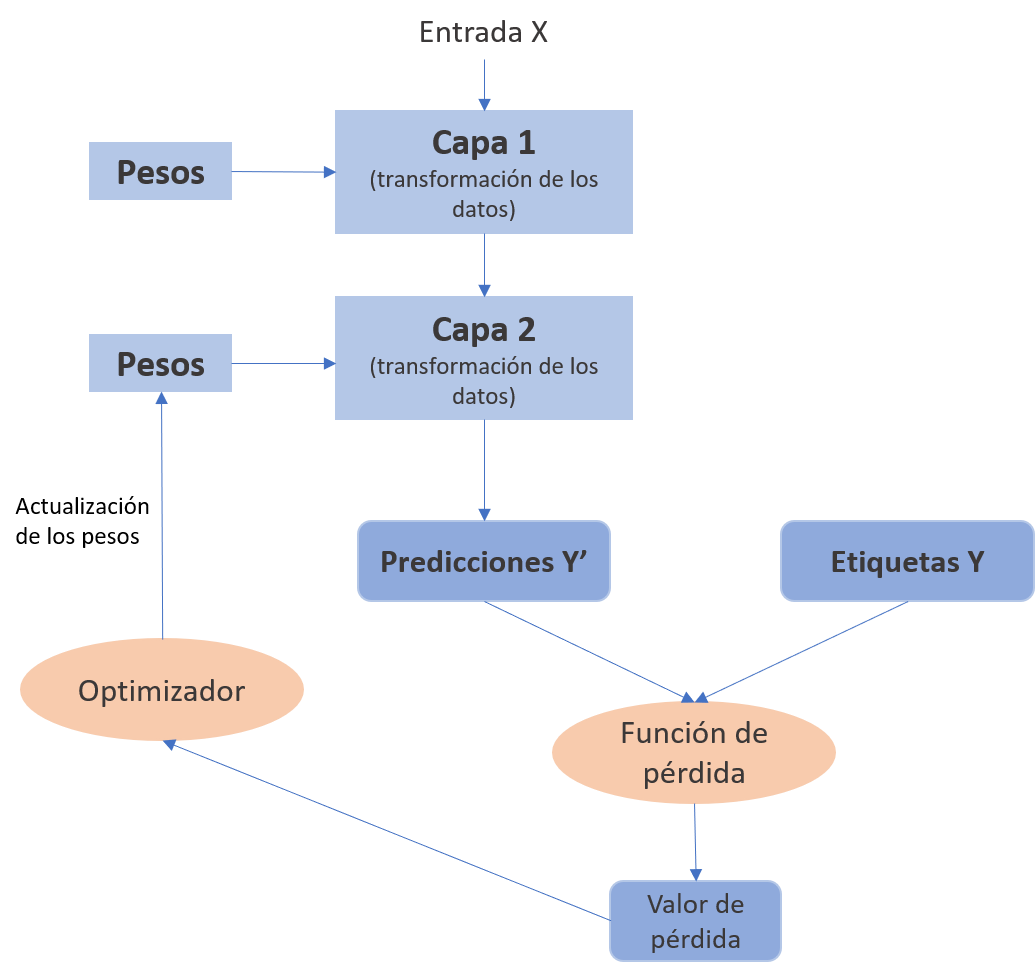
\includegraphics[width=3.8in]{Graphics/redBP.png}
	
	\caption{ \small{La pérdida es usada como señal de retroalimentación para el ajuste de los parámetros de la red.}}
	
	\label{RedBP}
	
\end{figure}

Inicialmente, los pesos de la red toman valores aleatorios mediante un proceso conocido como inicialización aleatoria (\textit{random initialization}).  Naturalmente, su salida está lejos de lo que debería ser, y en consecuencia, la medida de pérdida es muy alta. Pero con cada ejemplo que procesa la red, los pesos se ajustan un poco en la dirección correcta, y la pérdida disminuye. Este es el \textbf{ciclo de entrenamiento}, que, repetido las veces suficientes, produce valores de pesos que minimizan la función de pérdida. Las iteraciones comprendidas en el ciclo se conocen como épocas (\textbf{epochs}) del proceso de entrenamiento. Una red con una pérdida mínima es aquella donde la salida es lo más parecido posible al objetivo.
 %Nuevamente, es un mecanismo simple que, una vez escalado, termina pareciendo mágico.
 
 \subsection{Tipos de redes neuronales}\label{1-NN}
 
Una característica importante de algunas redes neuronales, como las \textbf{redes neuronales densamente conectadas}, es que no tienen memoria. Cada entrada a la misma se procesa de forma independiente, sin que se mantenga ningún estado de una entrada a otra. Para procesar una secuencia o una serie temporal de puntos en los datos, es necesario introducir de una vez la secuencia completa a la red. Tales redes se llaman redes unidireccionales (del inglés  \textit{feedforward} ). 

%feedforward -> unidireccionales

La predicción de datos secuenciales supone un problema en ML, ya que usualmente se analizan casos aislados como una imagen o un carácter que se desea clasificar. Sin embargo, lo que una persona entiende al ver una película o al mantener una conversación, se basa en conocimientos anteriores que van adquiriendo sentido con cada instante que transcurre. Las redes neuronales recurrentes (recurrent neural networks, RNN) son un tipo de algoritmo de aprendizaje profundo que se encarga de resolver este problema mediante el procesamiento de datos secuenciales \cite{BengioGood}.

Las RNN en lugar de tener una estructura por capas como las redes neuronales convencionales, poseen una estructura cíclica donde la salida de un estado pasa a ser la entrada del estado siguiente \ref{RNN} . Esto permite detectar dependencias temporales, es decir, dotar a la red de memoria (estado oculto o hidden state) para que retenga la información sobre lo calculado en la etapa anterior. De esta forma, utiliza los mismos parámetros para cada entrada, reduciendo así la complejidad de la red \cite{RNNVinyals}.

\begin{figure}[!h]
	
	\centering
	
	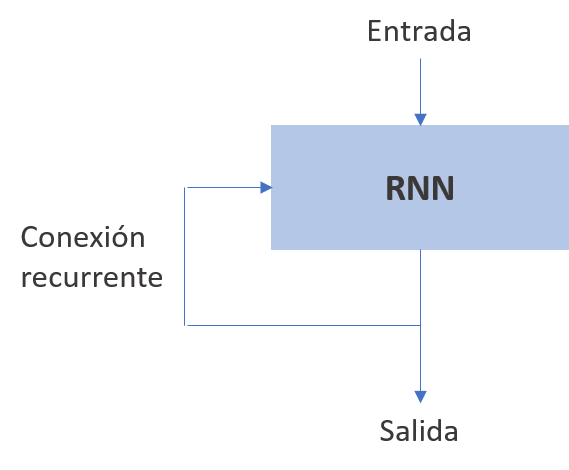
\includegraphics[width=2.3in]{Graphics/RNNConnection.png}
	
	\caption{\small{Esquema básico de una RNN}}
	\label{RNN}
	
\end{figure}

Como parte del amplio estudio realizado en esta tesis, se revisaron trabajos que incluyen la utilización de este tipo de redes \cite{SutskeverSeq2seqNN, PointerNVinyals}. Además, como se había mencionado, la solución propuesta en esta investigación contempla dos modelos de redes neuronales conocidos como \textit{autoencoder} y \textit{variational autoencoder}. Este último forma parte de los modelos generativos dentro del aprendizaje automático y se abordará en la siguiente sección.


\section{Modelos generativos}\label{1-GenModel}

Los modelos generativos constituyen un área del aprendizaje automático que se dedica a encontrar la distribución $P(X)$, definida sobre los puntos $X$ de un espacio $\mathcal{X}$ de gran dimensión. Por ejemplo, las imágenes son un tipo de datos muy popular empleadas en modelos generativos \cite{VAETutorial}, donde cada una puede tener miles o millones de píxeles. En este caso la tarea del modelo generativo es capturar de alguna manera las dependencias entre píxeles, por ejemplo, que los píxeles con colores similares se encuentren cercanos entre sí.

Un tipo sencillo de modelo generativo permite calcular numéricamente $P(X)$. En el caso de las imágenes, los valores $X$ que parecen imágenes reales deberían tener una alta probabilidad, mientras que las imágenes que posean determinado ruido aleatorio deberían tener una probabilidad baja.

 Su idea principal se basa en generar puntos nuevos, parecidos a los del conjunto de datos inicial, pero no exactamente los mismos. Formalmente, el objetivo es aprender un modelo $P$ para muestrear puntos $X$ que satisfacen una distribución no conocida $P^{*}(X)$, de forma tal que $P$ sea lo más parecido posible a $P^{*}$.
 
 Los \textit{variational autoencoders} constituyen un ejemplo clásico dentro de la familia de modelos generativos. Sus buenas propiedades de aproximación, y el pequeño error introducido con ella, aportan gran capacidad de generación al modelo. Además, son capaces de comprimir los datos de entrada en una representación con menos información, conocida como representación latente. Es por ello que su estudio resulta de gran interés en este trabajo.
 
  En el capítulo \ref{chapter:REV-LL} se profundizará en la teoría detrás del VAE y posteriormente, en el capítulo \ref{chapter:Solution} se explicará en qué consiste su uso para codificar soluciones del VRP a un vector real o vector latente. Antes de llegar a esos puntos, primeramente, se analizarán los modelos de variable latente en la siguiente sección. 
 
 
 %Dicho vector codificado, conocido también como vector de contexto o vector latente es analizado durante esta investigación, en cuanto a las propiedades y características capturadas de la distribución de entrada inicial. 
 


\subsection{Modelos de Variable Latente}\label{1-latentVarModel}

Los modelos matemáticos que tratan de explicar las variables observadas en términos de variables latentes se llaman modelos de variables latentes. Para comprender mejor en qué consisten, se presenta un ejemplo mediante el problema de la generación de imágenes referentes a dígitos escritos a mano.

 Durante el proceso, el modelo primeramente decide qué dígito va a generar antes de asignar valores a cualquiera de los píxeles. Este tipo de decisiones se conocen formalmente como variable latente. Es decir, el modelo muestrea aleatoriamente un dígito $z$ del conjunto $[0, ..., 9]$ y luego se asegura de que todos los trazos coincidan con el mismo. En este caso $z$ es la variable latente. A continuación se define formalmente.
 
 Si $z$ es un vector de variable latente en un espacio de dimensión elevada $\mathcal{Z}$, $z$ puede ser muestreado de acuerdo a la función de densidad probabilística $P(z)$ definida sobre $\mathcal{Z}$. También se tiene a $f(z; \theta)$ como una familia de funciones deterministas parametrizadas por un vector $\theta$ que pertenece a un espacio $\Theta$, donde $f: \mathcal{Z} \times \Theta \rightarrow X$.
 
  Como $f$ es determinista y $\theta$ no lo es, entonces $f(z; \theta)$ es una variable aleatoria en el espacio $\mathcal{X}$. La idea es optimizar los parámetros $\theta$ de forma tal que se pueda muestrear $z$ a través de $P(z)$, teniendo en cuenta que $f(z; \theta)$ serán como los elementos $X$ del conjunto de datos. 
 
 Matemáticamente el objetivo es maximizar la probabilidad de cada punto $X$ en el conjunto de entrenamiento a lo largo del proceso generativo, de acuerdo a:
 
 \begin{equation}
 	P(X) = \displaystyle{\int} P(X| z; \theta)P(z)dz
 \end{equation} 
 
 Aquí, $f(z; \theta)$ se reemplazó por una distribución $P(X| z; \theta)$, lo que permite hacer explícita la dependencia de $X$ con $z$ utilizando la ley de probabilidad total. En los modelos VAEs la función de distribución empleada generalmente  es Normal, es decir $P(X|z;\theta) = \mathcal{N}(X|f(z; \theta), \sigma^2*I)$. La media se define a partir de $f(z, \theta)$ y la covarianza como la matriz identidad $I$ multiplicada por un escalar $\sigma$ (que es un hiperparámetro de la red neuronal). Estas sustituciones son necesarias para formalizar la intuición de que las variables $z$ necesitan ser parecidas a algún $X$ \cite{VAETutorial}. 
 
 En general, y particularmente al principio del entrenamiento, el modelo no producirá resultados que sean idénticos a cualquier $X$ en particular. Al tener una distribución gaussiana, se usa descenso por gradiente para aumentar la probabilidad $P(X)$, haciendo que $f(z; \theta)$ se aproxime a $X$ para algún $z$, es decir, permitiendo gradualmente que los datos de entrenamiento sean más probables bajo el modelo generativo.\\
 
 Con este primer capítulo se presentó una introducción al aprendizaje automático. En esencia, se ofrecieron los principios y conceptos teóricos más importantes del área que fundamentan el trabajo realizado en esta tesis y muchas de las decisiones tomadas. Aprender a resolver automáticamente problemas complejos como el VRP, podría implicar el próximo salto en el desarrollo de la optimización combinatoria.  
 
 La solución propuesta en este trabajo para codificar soluciones del VRP a vectores de un espacio continuo, tiene lugar en este terreno. Específicamente mediante el uso de los modelos \textit{autoencoders} y \textit{variational autoencoders}. En el próximo capítulo se profundiza en la definición teórica de estos modelos de redes neuronales, así como también las aplicaciones de los mismos en problemas de codificación similares. También se exponen una serie de técnicas de ML que resultan de gran interés para esta investigación. 
 
 
 
 
 




 

